% =====================================================================
% Preliminary Paper — Analyzing Hallucination Patterns in RAG-Based
% Financial Question Answering (CS6120 NLP, Northeastern University)
%
% Uses the provided ACL 2023 template (paper/templates/acl2023/).
% To compile: place this file next to acl2023.sty and acl_natbib.bst
% (both in templates/acl2023/), with references.bib, fig_eda_overview.png,
% and results_table.tex in the same folder — all are copied into paper/.
% Build: pdflatex main -> bibtex main -> pdflatex main x2.
% For the final (non-anonymous) look we drop the [review] option.
% =====================================================================
\pdfoutput=1
\documentclass[11pt]{article}
\usepackage{acl2023}        % provided template style (templates/acl2023/acl2023.sty)
\usepackage{times}
\usepackage{latexsym}
\usepackage[T1]{fontenc}
\usepackage[utf8]{inputenc}
\usepackage{microtype}
\usepackage{graphicx}
\usepackage{booktabs}

\title{Analyzing Hallucination Patterns in Retrieval-Augmented\\
Financial Question Answering: A Preliminary Study}

\author{
  Bhalchandra Shinde \and Piyush Daga \and Anish Kelkar \and Rituraj Singh \\
  Khoury College of Computer Sciences, Northeastern University \\
  \texttt{\{shinde.b, daga.p, kelkar.a, singh.rit\}@northeastern.edu}
  % TODO: verify the exact NEU usernames for Piyush (daga.p?) and Rituraj (singh.rit?)
}

\begin{document}
\maketitle

\begin{abstract}
Retrieval-augmented generation (RAG) grounds large language models (LLMs) in
external documents, yet models still produce claims that contradict or exceed
the retrieved evidence---a failure mode with acute consequences in finance,
where a single wrong figure misleads. We study \emph{when and how} RAG systems
hallucinate on financial QA using the open-source subset of
\textbf{FinanceBench} (150 annotated questions over 84 SEC filings). This
preliminary report contributes: (i) an expanded literature review situating our
work across RAG methods, hallucination evaluation, and financial NLP; (ii) an
exploratory analysis showing that FinanceBench answers are overwhelmingly
\emph{abstractive}---only 2\% appear verbatim in the cited evidence---over long,
table-heavy 10-K filings, precisely the regime where grounded generation is
hard; and (iii) a simple baseline pipeline (BM25 + GPT-3.5-turbo) evaluated with
RAGAS faithfulness and token-level F1/Exact Match. Our results establish a
working end-to-end system and quantify the retrieval bottleneck that drives both
abstention and the ``grounded-but-wrong'' errors we will taxonomize in the final
paper.
\end{abstract}

\section{Introduction}
Retrieval-augmented generation~\citep{lewis2020rag} has become the dominant
recipe for grounding LLM outputs in verifiable external knowledge. Yet a growing
body of work shows that even with relevant context in the prompt, models
generate statements that are unsupported by---or contradict---the retrieved
passages~\citep{ji2023hallucination,huang2023hallucinationsurvey}. In
\emph{financial} question answering this is especially costly: answers are exact
numeric values drawn from dense regulatory filings, and a single fabricated or
misattributed figure produces a confidently wrong answer.

We investigate three research questions:
\begin{itemize}
  \item[\textbf{RQ1}] How frequently do different RAG pipeline configurations
  hallucinate on financial QA?
  \item[\textbf{RQ2}] Which hallucination \emph{types} dominate in finance---
  numerical, entity, reasoning, or unsupported extrapolation?
  \item[\textbf{RQ3}] Do larger / instruction-tuned LLMs hallucinate less given
  the same retrieved context?
\end{itemize}

This report establishes the foundation for answering them: a literature review
(\S\ref{sec:related}), an exploratory analysis of FinanceBench that motivates
the difficulty (\S\ref{sec:data}), and a working baseline pipeline with
preliminary faithfulness and accuracy metrics (\S\ref{sec:results}). We close
with the roadblocks this early evidence surfaces (\S\ref{sec:next}).%
\footnote{\textbf{Contributions.} Bhalchandra Shinde: repository/infrastructure,
environment, data pipeline, exploratory data analysis, and literature-review
notes for \citet{lewis2020rag} and \citet{islam2023financebench}. Anish Kelkar:
document chunking, baseline RAG pipeline, evaluation harness (RAGAS + F1/EM), and
results tabulation. Piyush Daga and Rituraj Singh: remaining related-work papers
and paper writing. All members contributed to the final draft.}

\section{Related Work}
\label{sec:related}
We organize related work into three themes: RAG methods and retrieval,
hallucination detection and evaluation, and financial NLP/QA.

\paragraph{RAG methods and retrieval.}
RAG was introduced by \citet{lewis2020rag}, coupling a DPR retriever with a BART
generator and framing knowledge as \emph{parametric} (model weights) versus
\emph{non-parametric} (an editable document index) memory; it is the
architectural baseline our pipelines instantiate. Two of its findings bear
directly on our setting. First, RAG answers correctly even when the gold answer
appears in \emph{no} retrieved passage verbatim (11.8\% of Natural Questions
cases), where a purely extractive reader scores zero---the same
\emph{abstractive} regime we observe in FinanceBench, where only 2\% of gold
answers are verbatim in the evidence (\S\ref{sec:data}). Second, swapping the
document index updates the model's world knowledge with no retraining,
underscoring that retrieval quality---not generator memory---governs what a RAG
system can ground, which is precisely the bottleneck our results expose.
The two retrieval families we compare are defined by
BM25~\citep{robertson2009bm25}, a probabilistic term-matching function that is
our baseline retriever, and DPR~\citep{karpukhin2020dpr}, which learns dense
question/passage encoders and beats BM25 on most open-domain QA---motivating our
planned dense pipeline. That dense pipeline embeds chunks with
Sentence-BERT~\citep{reimers2019sbert}, a siamese-BERT model that produces
semantically comparable sentence vectors, the encoder behind our MiniLM index.
REALM~\citep{guu2020realm} pre-trains the retriever jointly with a masked LM, and
Fusion-in-Decoder~\citep{izacard2021fid} instead fuses many retrieved passages in
the decoder; both integrate retrieval more deeply than our prompt-based setup and
mark upgrade paths we may explore.
Self-RAG~\citep{asai2024selfrag} trains a model to decide \emph{when} to retrieve
and to critique its own generations with reflection tokens---directly relevant to
cutting the unsupported answers we aim to reduce.
Query rewriting~\citep{ma2023queryrewriting} expands or reformulates the query
before retrieval and is exactly the mechanism of our planned ``enhanced''
pipeline. The recent survey of \citet{gao2023ragsurvey} organizes these advances
and motivates our controlled comparison of retrieval strategies.

\paragraph{Hallucination detection and evaluation.}
\citet{ji2023hallucination} and \citet{huang2023hallucinationsurvey} survey
hallucination in NLG and LLMs respectively and provide the vocabulary
(intrinsic vs.\ extrinsic, faithfulness vs.\ factuality) our taxonomy refines
for finance. For measurement, RAGAS~\citep{es2024ragas} supplies reference-free
metrics---faithfulness, answer relevancy, context precision---that we adopt as
our primary hallucination signal. SelfCheckGPT~\citep{manakul2023selfcheckgpt} detects hallucination without
external resources by sampling several responses and measuring their mutual
consistency, while FActScore~\citep{min2023factscore} decomposes a generation
into atomic facts and scores each against a source---two complementary detection
lenses we consider for the final error analysis.
RAGTruth~\citep{niu2024ragtruth} contributes a word-level hallucination corpus
and taxonomy that we will use as supervision for the (optional) automatic
classifier, and the RGB benchmark~\citep{chen2024rgb} evaluates LLM robustness
to noisy retrieval---the ``wrong context'' condition our full-corpus retriever
deliberately induces. We additionally report token-level F1/EM following the
SQuAD protocol~\citep{rajpurkar2016squad} to capture correctness that
faithfulness alone misses, and note RAGBench~\citep{friel2024ragbench} as a
cross-domain resource for future comparison.

\paragraph{Financial NLP and QA.}
FinanceBench~\citep{islam2023financebench} is our primary benchmark: 10{,}231
open-book questions over 361 real 10-K/10-Q/8-K/earnings filings from 40 US
companies, of which a human-reviewed 150-question subset (the open-source
release) is our evaluation set. Its own experiments motivate our study in three
ways. (i)~66\% of its questions require \emph{numerical reasoning} rather than
extraction---our EDA independently recovers this numeric skew (\S\ref{sec:data}).
(ii)~Even the best realistic configuration (GPT-4-Turbo, long context) reaches
only $\sim$79\% accuracy against an 85\% oracle ceiling, and confident
\emph{hallucination} is a named failure theme---the phenomenon we set out to
quantify and taxonomize. (iii)~They report that stronger models tend to
\emph{refuse} when uncertain while weaker ones answer wrong; our GPT-3.5 baseline
likewise abstains rather than fabricate (\S\ref{sec:results}), and they find
placing context \emph{before} the question is critical---a design choice our
prompt template adopts.
Prior financial QA datasets establish that numerical reasoning over hybrid
table/text is the core difficulty our EDA also finds:
FinQA~\citep{chen2021finqa} pairs expert-written questions with executable
reasoning programs over earnings-report tables;
ConvFinQA~\citep{chen2022convfinqa} extends this to multi-turn conversational
chains; and TAT-QA~\citep{zhu2021tatqa} targets questions that jointly span a
table and its surrounding text---exactly the table+prose evidence our chunker
must preserve. On the model side, BloombergGPT~\citep{wu2023bloomberggpt}, a 50B
model pre-trained on a large financial corpus, and FinGPT~\citep{yang2023fingpt},
an open finance-LLM framework, show the appetite for finance-specialized models
but evaluate generation quality rather than isolating \emph{RAG} hallucination,
which is our focus. Our open-source generator comparison will use
Mistral-7B-Instruct~\citep{jiang2023mistral}, a strong 7B open model, as the RQ3
counterpart to GPT-3.5. Collectively, this line of work motivates a
finance-specific, RAG-centric hallucination study---the gap our project targets.

\section{Data and Exploratory Analysis}
\label{sec:data}
\textbf{Dataset.} We use the open-source subset of
FinanceBench~\citep{islam2023financebench}: 150 QA pairs spanning 32 companies
and 84 source filings (fiscal years 2015--2024) across 9 GICS sectors. Question
types are balanced by design (50 metrics-generated, 50 domain-relevant, 50
novel-generated). Each record carries a gold answer and an evidence span, letting
us judge groundedness directly.

\textbf{Findings.} Figure~\ref{fig:eda} summarizes the analysis
(full notebook and 22 figures in the repository). Four properties make this a
stress test for grounded generation:
(1)~\emph{Long, tabular context}---source filings have a median of 128 pages and
evidence spans are 69\% table-heavy, so retrieval operates over large, noisy
documents.
(2)~\emph{Short, numeric answers}---the median gold answer is 9 words and 84\%
are numeric, so a single wrong figure flips a correct answer to wrong.
(3)~\emph{Abstractive answers}---only 2\% of gold answers appear \emph{verbatim}
in the evidence (mean extractability 0.27); the model must \emph{synthesize} a
value, not copy it, which is the core hallucination risk.
(4)~\emph{Modest lexical overlap}---median question--evidence cosine similarity
is 0.47, so retrievers must bridge a vocabulary gap, and 46\% of questions
require numerical computation or aggregation. These observations justify
measuring faithfulness (RAGAS) alongside F1/EM and motivate our four-category
hallucination taxonomy.

\begin{figure}[t]
  \centering
  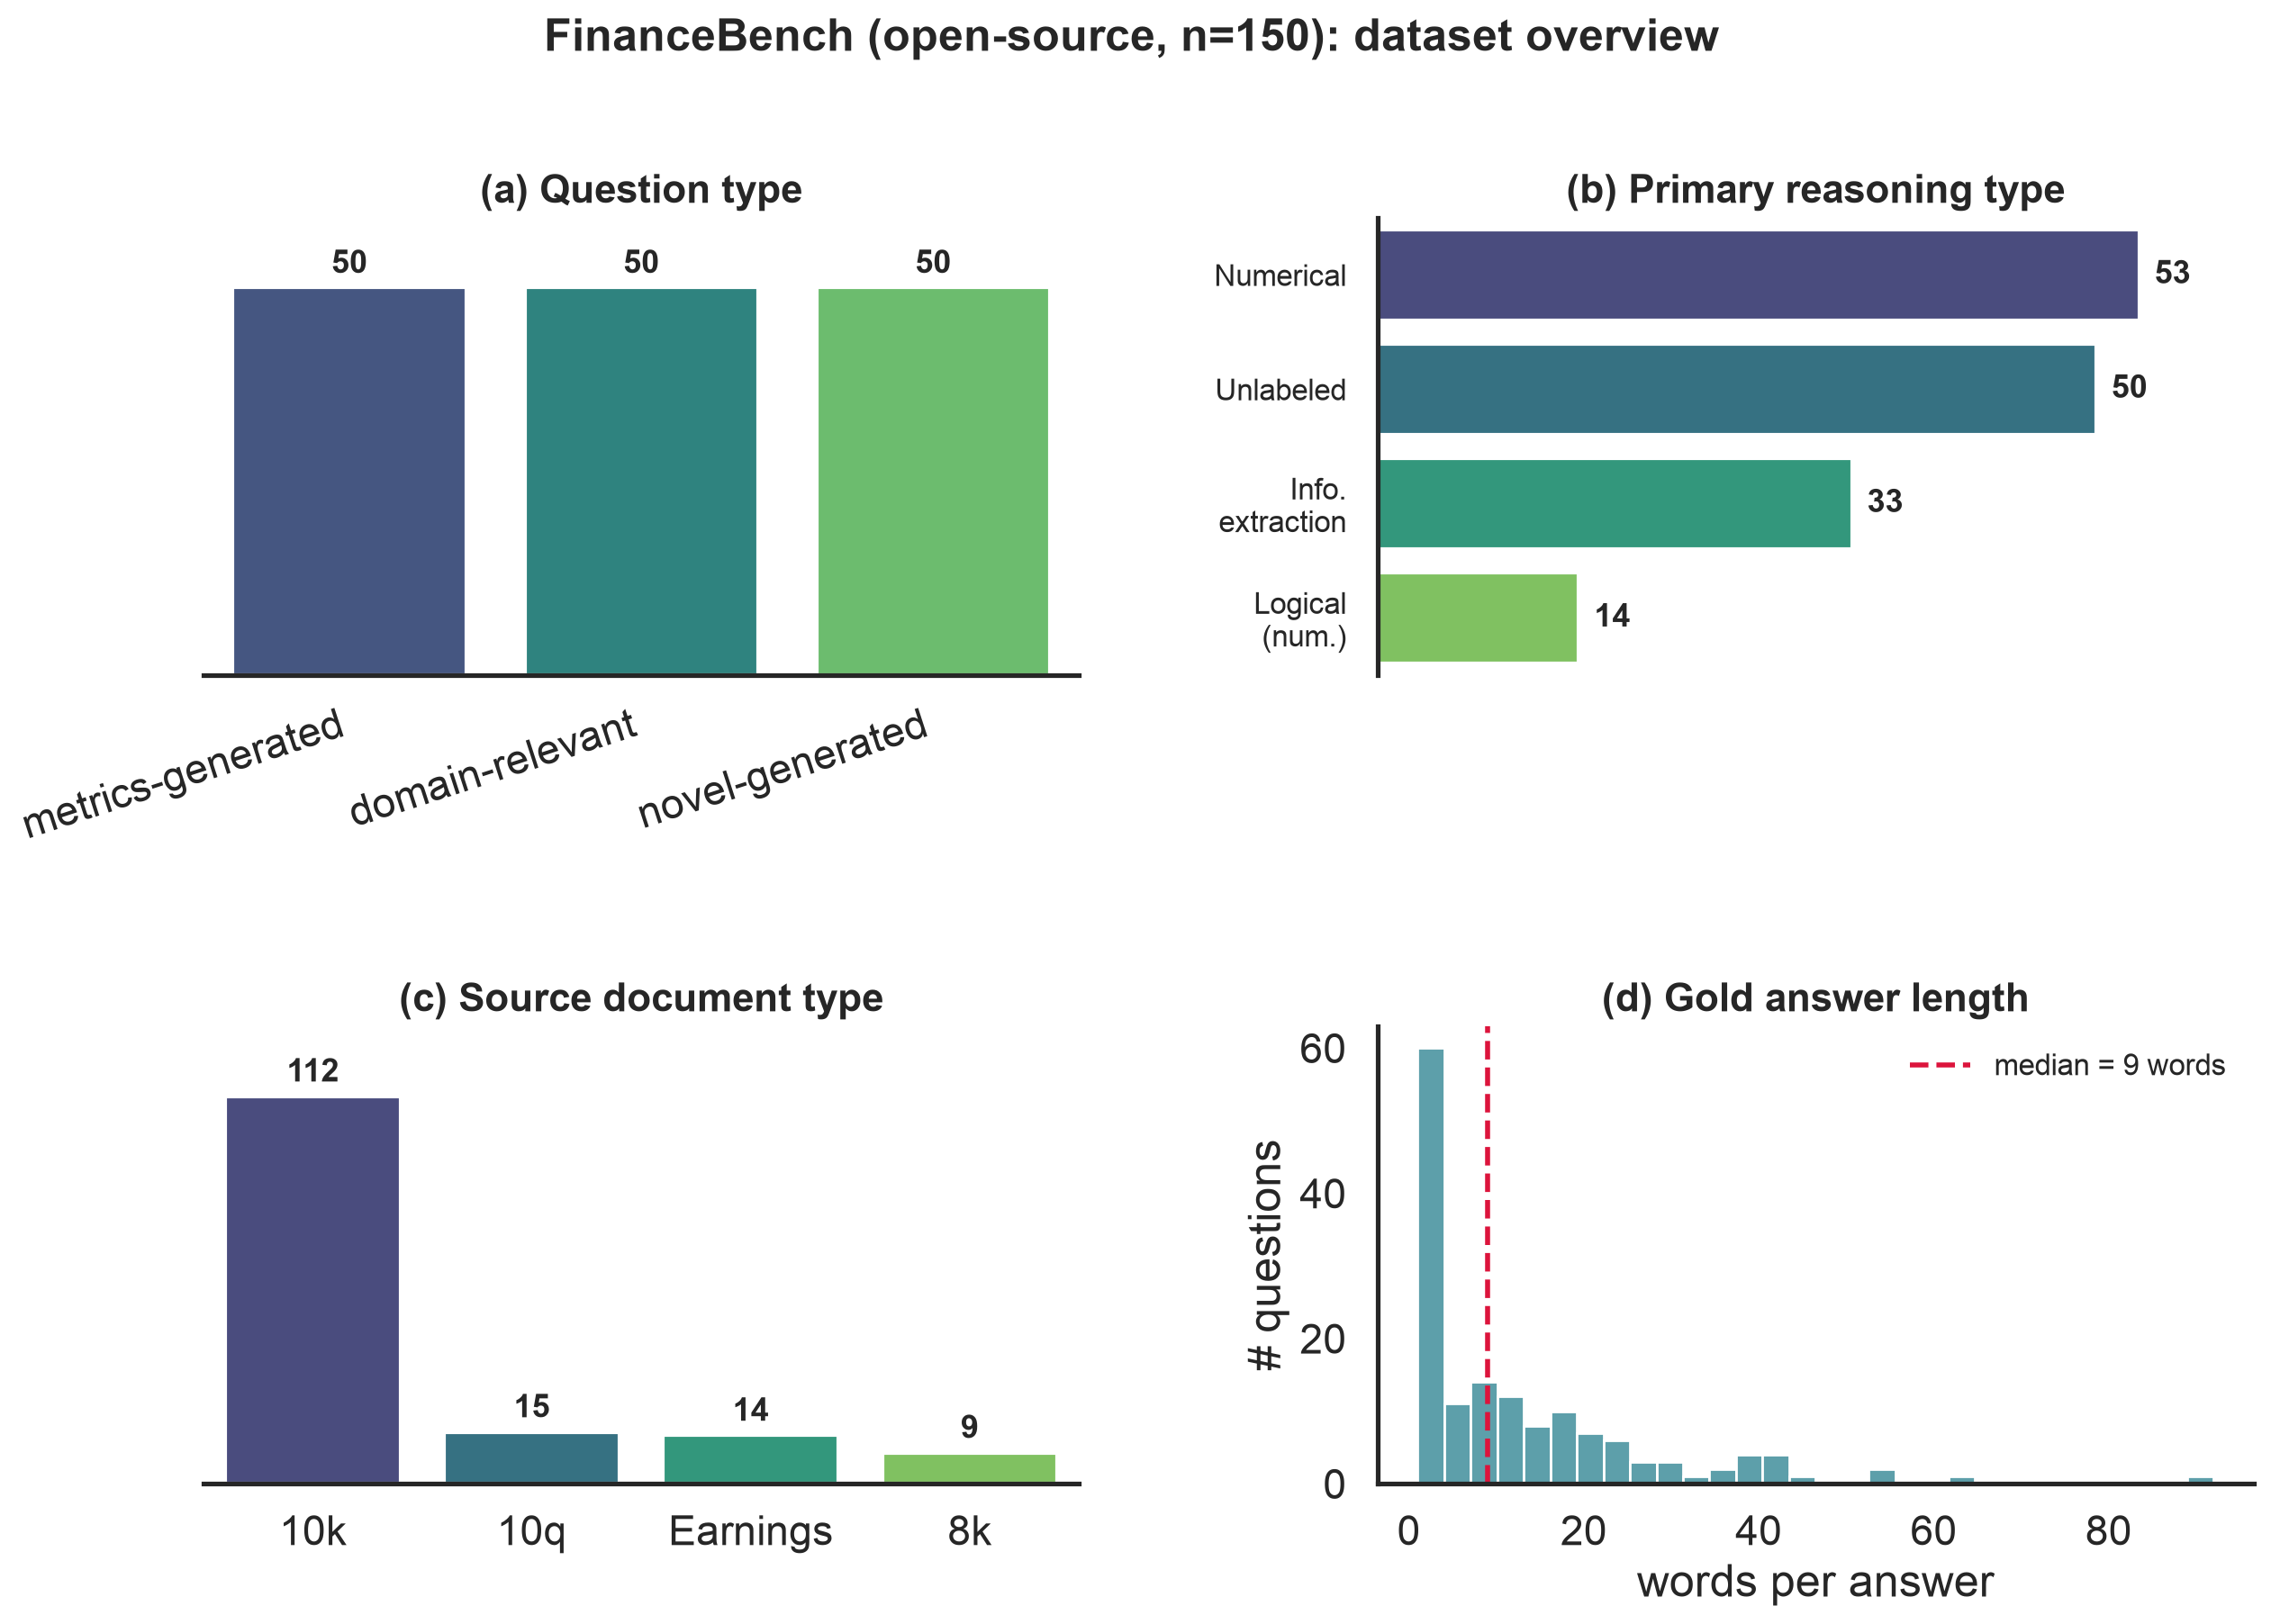
\includegraphics[width=\columnwidth]{fig_eda_overview.png}
  \caption{FinanceBench (open-source, $n{=}150$) overview: (a) balanced question
  types, (b) numeric reasoning dominates, (c) 10-K filings dominate the corpus,
  (d) gold answers are short. See \S\ref{sec:data}.}
  \label{fig:eda}
\end{figure}

\section{Preliminary Method and Results}
\label{sec:results}
\textbf{Pipelines.} All configurations share the same GPT-3.5-turbo generator
(temperature 0), prompt, 512-token chunks, and top-3 retrieval; only
\emph{retrieval} changes, which isolates its effect. We compare \emph{Baseline}
(BM25 sparse retrieval over the entire 84-filing corpus), \emph{Dense} (FAISS over
MiniLM embeddings), and \emph{Enhanced} (an LLM rewrites the query before dense
retrieval), plus a known-document upper bound (\emph{Single-doc}: retrieval
restricted to the question's own filing). We index the full corpus on purpose---a
retriever that can surface the \emph{wrong} filing among 84 is exactly where
hallucination appears. The prompt instructs the model to answer only from context
and to say ``I don't know'' when the answer is absent, so a wrong answer is a
grounding failure rather than a memory guess. A fixed output schema lets one
harness score every pipeline.

\textbf{Evaluation.} We report RAGAS~\citep{es2024ragas} faithfulness, answer
relevancy, and context precision (LLM judge: GPT-4o-mini; local
sentence-transformer embeddings), plus SQuAD-style token F1 and Exact
Match~\citep{rajpurkar2016squad}. Because gold answers are short numbers formatted
many ways (\$1{,}577 vs.\ 1577.00 vs.\ 1.577 billion), strict EM is near zero, so we
also report a \emph{numeric-tolerant} EM (right value within 1\%, ignoring format)
and faithfulness on the \emph{answered} subset. Retr@3 is the share of questions
whose top-3 retrieval reached the correct filing.

\begin{table*}[t]
\centering
\small
\caption{Retrieval-strategy comparison on FinanceBench (all 150 questions). Retr@3 = share of questions whose top-3 retrieval surfaced the correct filing; Faith(ans) = faithfulness over answered questions only; EM(num) = numeric-tolerant exact match. Generator + query-rewriter = GPT-3.5-turbo (temp 0); RAGAS judge = GPT-4o-mini; embeddings = MiniLM (\texttt{all-MiniLM-L6-v2}).}
\label{tab:pipeline-comparison}
\begin{tabular}{lrrrrrrrr}
\toprule
Pipeline & Retr@3 & Faithful. & Faith(ans) & Ans. Rel. & Ctx. Prec. & Answered & F1 & EM (num) \\
\midrule
Baseline (BM25) & 43\% & 0.104 & 0.408 & 0.234 & 0.240 & 47/150 & 0.083 & 0.120 \\
Dense (FAISS) & 64\% & 0.197 & 0.352 & 0.414 & 0.417 & 82/150 & 0.116 & 0.180 \\
Enhanced (rewrite) & 69\% & 0.209 & 0.353 & 0.432 & 0.462 & 87/150 & 0.121 & 0.207 \\
Dense, single-doc & 100\% & 0.300 & 0.572 & 0.424 & 0.435 & 96/150 & 0.139 & 0.267 \\
\bottomrule
\end{tabular}
\end{table*}


\textbf{Results.} Every metric improves as retrieval improves
(Table~\ref{tab:pipeline-comparison}). The correct filing reaches the top-3 for
\textbf{43\% $\rightarrow$ 64\% $\rightarrow$ 69\%} of questions
(BM25 $\rightarrow$ dense $\rightarrow$ rewrite); because the model answers only from
context, coverage rises in lockstep (\textbf{47 $\rightarrow$ 82 $\rightarrow$ 87} of
150), and so do context precision ($0.24 \rightarrow 0.42 \rightarrow 0.46$),
faithfulness ($0.10 \rightarrow 0.20 \rightarrow 0.21$), token F1
($0.083 \rightarrow 0.116 \rightarrow 0.121$), and numeric-tolerant EM
($0.12 \rightarrow 0.18 \rightarrow 0.21$). Since only retrieval changed, this isolates
\textbf{retrieval as the dominant lever (RQ1)}. Strict EM $\approx$0 understates
accuracy: the numeric-tolerant EM shows 33--42\% of \emph{answered} questions are
actually correct---the model was penalized for formatting, not errors. Faithfulness is
low overall, but that is dominated by abstentions (an ``I don't know'' has nothing to
ground); on the answered subset it is moderate (0.35--0.57), i.e.\ when the model
commits to an answer it is partly---not fully---grounded, which is precisely the
hallucination we study. The known-document upper bound makes the ceiling explicit:
restricting retrieval to the correct filing lifts Retr@3 to 100\%, coverage to 96/150,
F1 to 0.139, and answered-faithfulness to 0.57---yet a third of questions still go
unanswered, so finding the right filing is necessary but not sufficient. Those
answered-but-unsupported cases are exactly what our error analysis will taxonomize.

\section{Roadblocks and Next Steps}
\label{sec:next}
The preliminary run isolates the key bottleneck: sparse full-corpus retrieval
often fails to surface the correct filing, so the model either abstains or
answers from wrong context. This directly shapes our plan: (1)~dense retrieval
(FAISS + sentence embeddings) and query rewriting to raise retrieval recall
(RQ1); (2)~an open-source generator (Mistral-7B~\citep{jiang2023mistral}) under
the same retrieval config to test RQ3; and (3)~manual annotation of 50 failure
cases into our four-type taxonomy (numerical, entity, reasoning, unsupported
extrapolation) to answer RQ2. The main risks are OpenAI API cost control (run
once at temperature 0) and the fidelity of PDF table extraction, which flattens
tables into linear text and is a known limitation we will quantify.

\bibliography{references}
\bibliographystyle{acl_natbib}

\appendix
\section{Additional EDA Figures}
The repository includes 22 EDA figures (question/answer/evidence/source-document
distributions, retrieval-difficulty and hallucination-risk proxies, and
linguistic-complexity analyses) generated by \texttt{notebooks/01\_eda.ipynb}.

\end{document}
